% ISCA 2027 main-track submission (template: template/, the ISCA 2026 IEEE package, IEEEtran.cls unchanged).
% Format: at most 11 pages of two-column text NOT counting references (references unlimited, 8 pt); US letter;
% 10 pt Times body, 8 pt captions; page numbers on every page; the submission banner on page 1; double-blind (no
% author names in the text or the PDF metadata); every reference lists ALL its authors (no "et al.").
\documentclass[conference]{IEEEtran}
\IEEEoverridecommandlockouts
\usepackage{cite}
\usepackage{amsmath,amssymb,amsfonts}
\usepackage{graphicx}
\usepackage{textcomp}
\usepackage{booktabs}
\usepackage{array}% >{\raggedright} columns (Table cmds)
\usepackage{xcolor}
\usepackage{xspace}
\usepackage{pifont}% circled step numbers (\ding{172} = 1) keyed to Fig. tile
% clickable figure, table, section and citation numbers; one dark blue that still reads in print; loaded last
\definecolor{linkblue}{RGB}{0,51,153}
\PassOptionsToPackage{hyphens}{url}% long web URLs in the bibliography break at hyphens
\usepackage[colorlinks,linkcolor=linkblue,citecolor=linkblue,urlcolor=linkblue]{hyperref}
% double-blind: the PDF metadata carries the paper title only, never an author
\hypersetup{pdftitle={Commands Are the Bottleneck: CoDe, a Command-Decoupled PIM for Skinny GEMMs on Mobile and Server DRAM},
  pdfauthor={}, pdfsubject={}, pdfkeywords={}}

% ---- macros -----------------------------------------------------------------
% a value still being computed by another owner; must be 0 at submission
\newcommand{\PENDING}[1]{\textcolor{red}{\textbf{[PENDING: #1]}}}
% an unavoidable modelling assumption (project rule: every assumption is tagged)
\newcommand{\ASSUMPTION}{\textsuperscript{\textsc{[assumption]}}}
\newcommand{\tccds}{$t_\mathrm{CCD\_S}$\xspace}
\newcommand{\tccdl}{$t_\mathrm{CCD\_L}$\xspace}
\newcommand{\tcol}{$t_\mathrm{col}$\xspace}
% useful-MAC utilization (III-B; the symbols work in and out of math, xspace only in text): U = U_MAC x f_MAC; canonical names "useful-MAC utilization U", "slot factor",
% "sweep factor", "row sweep", "row-switch commands" / "row-switch overhead" (t_row), "token load/drain commands" (t_tok),
% "beat filling", "row reuse" (D-36); never "PU busy" or "PU utilization" (retired 2026-10-19)
\newcommand{\tck}{\ensuremath{t_\mathrm{CK}}\ifmmode\else\expandafter\xspace\fi}
\newcommand{\tslot}{\ensuremath{t_\mathrm{slot}}\ifmmode\else\expandafter\xspace\fi}
\newcommand{\trow}{\ensuremath{t_\mathrm{row}}\ifmmode\else\expandafter\xspace\fi}
\newcommand{\ttok}{\ensuremath{t_\mathrm{tok}}\ifmmode\else\expandafter\xspace\fi}
\newcommand{\UMAC}{\ensuremath{U_\mathrm{MAC}}\ifmmode\else\expandafter\xspace\fi}
\newcommand{\fMAC}{\ensuremath{f_\mathrm{MAC}}\ifmmode\else\expandafter\xspace\fi}

\begin{document}
\bstctlcite{IEEEexample:BSTcontrol}

% Ensure letter paper
\pdfpagewidth=8.5in
\pdfpageheight=11in

%%%%%%%%%%%---SETME-----%%%%%%%%%%%%%
\newcommand{\iscasubmissionnumber}{NaN}
%%%%%%%%%%%%%%%%%%%%%%%%%%%%%%%%%%%%

\pagenumbering{arabic}

\title{Commands Are the Bottleneck: CoDe, a Command-Decoupled PIM for Skinny GEMMs on Mobile and Server DRAM}
\author{\normalsize{ISCA 2027 Submission
    \textbf{\#\iscasubmissionnumber} -- Confidential Draft -- Do NOT Distribute!!}}

\maketitle
\thispagestyle{plain}
\pagestyle{plain}

% Abstract: seven moves, <= 200 words; every number also printed in Sec. I or II.
\begin{abstract}
Large language model decoding on mobile platforms and edge servers runs skinny GEMMs: speculative decoding verifies a few
drafted tokens and batching serves a few requests, so each weight matrix meets 2 to 32 tokens and the host stays memory-bound. DRAM processing-in-memory (PIM) offers the bandwidth but is
designed for GEMV: its processing units (PUs) run one multiply--accumulate (MAC) beat per column command, so their
compute serves one token, not 32. Prior designs keep every MAC paced by a DRAM command: LP-Spec widens each command's
MAC step with 4$\times$ the multipliers, and P3-LLM's command per token caps a read at two tokens. We observe that
DRAM timing parameters bound column accesses, not MACs on a latched column: a column lasts 5\,ns on LPDDR5-6400 and
4\,ns on HBM2, and each period fits four PU beats at 0.8--1\,GHz. We propose CoDe (Command-Decoupled PIM): one
command delivers a weight column, which the PU applies to a tile of tokens at its own clock. On each rival's
memory, workload and precision, CoDe reaches 1.86$\times$ LP-Spec-style's GEMM throughput per logic mm$^2$ at the
same decode speed (1.00--1.006$\times$) on a mobile platform, and on HBM2 runs batched decode steps 1.68$\times$
faster than P3-LLM-style at 1.26$\times$ its throughput per logic mm$^2$ and 1.64$\times$ its system energy efficiency.
\end{abstract}

\section{Introduction}
\label{sec:intro}

% P:intro-skinny-gemm
Large language models (LLMs) now decode on mobile platforms and on edge servers, where the decode step is set by how many tokens share one pass over the weights. A mobile platform such as a smartphone runs speculative decoding: a small draft model proposes tokens and the target model verifies the drafted tokens in one pass~\cite{leviathan2023,sdnpu,lpspec}. An edge server batches a few requests per
step~\cite{p3llm}. Either way, each linear layer runs a skinny GEMM~\cite{flashdecodingpp}: the layer multiplies a weight matrix whose
dimensions are in the thousands by $M$ token vectors, with $M$ from 2 to about 32.

% P:intro-host-memory-bound
On the host, a skinny GEMM costs about what a GEMV costs. The host streams every weight once per step and performs $2M$
operations per weight, so the host stays memory-bound until $M$ reaches its ridge point at $M \approx 143$ for a Snapdragon 8 Gen 3~\cite{sd8g3}
NPU reading LPDDR5-6400 at 42\,GB/s (Section~\ref{sec:bg:roofline}).

% P:intro-pim-gemv-ceiling
DRAM processing-in-memory (PIM) removes the bandwidth limit but adds a compute ceiling built for GEMV. AiM-style PIM (Fig.~\ref{fig:dram_pim}a)
places a processing unit (PU) beside each bank and reads all banks with one column command~\cite{aimjssc,hbmpim}, for 9.75$\times$ the host's bandwidth on the mobile platform and 4$\times$ on HBM2. Each column command, however, drives one
multiply--accumulate (MAC) beat per PU (Fig.~\ref{fig:dram_pim}b), so a skinny GEMM costs $M$ GEMVs. Stock AiM-style PIM therefore wins a whole
decode step against the host only up to $M = 6$ on the mobile platform and $M = 2$--3 on HBM2 (Fig.~\ref{fig:roofline}).
Published systems send skinny GEMMs back to the host~\cite{attacc,neupims,ianus,p3llm}.

% float placed early: column-width schematic (Section II-B), defined here, past the point where it would
% still fit in page 1's left column, so it renders at the top of the right column
\begin{figure}[t]
  \centering
  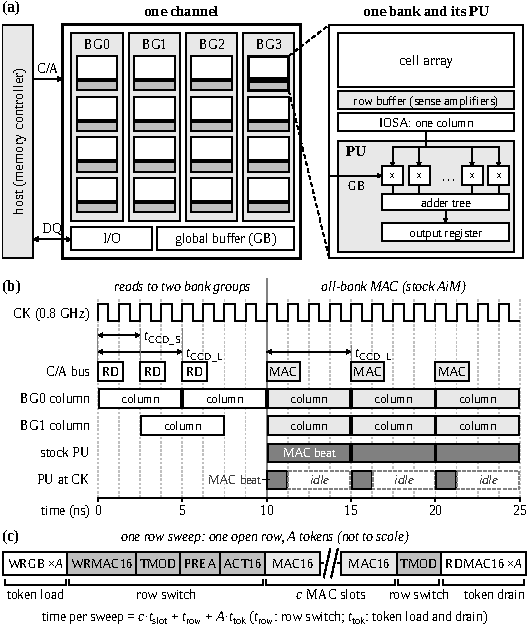
\includegraphics[width=\columnwidth]{figs/fig_dram_pim.pdf}
  \caption{AiM-style PIM: (a)~one channel and one bank with its PU; (b)~commands and MAC beats on the mobile platform; (c)~one row sweep.}
  \label{fig:dram_pim}
\end{figure}

% P:intro-prior-families
Prior PIM designs raise the ceiling in two families, and each family keeps every MAC paced by a DRAM command. The wider-PU
family spends multipliers: LP-Spec~\cite{lpspec} keeps one MAC step per column command and widens the step, feeding one
read to four 32-wide ALUs. The four ALUs carry four times the multipliers, and LP-Spec~\cite{lpspec} estimates that its
compute units and buffers take 16.92\,\% of an LPDDR5 die. The faster-PU family spends commands: P3-LLM~\cite{p3llm}
latches a weight and issues one command per token, so P3-LLM's MACs inherit the minimum command spacing \tccds, half the
column period: at most two tokens share a read.

% P:intro-timing-insight
Critically, DRAM timing parameters exist to meet DRAM access requirements by spacing the column commands that move data
out of the cell array~\cite{hbmpim}, not the MACs on a column already latched beside the bank. The column period
$t_\mathrm{col}$, the time one all-bank column command occupies the bank, sets how often a column arrives, and the PU
clock $f_\mathrm{PU}$ sets how often the PU computes, so one column can feed $D = t_\mathrm{col} \times f_\mathrm{PU}$
beats. An all-bank column lasts 5\,ns on LPDDR5-6400~\cite{lpspec} and 4\,ns on HBM2~\cite{hbmpim}, and a PU built in a
DRAM process runs at 1\,GHz in silicon~\cite{aimjssc}. A PU clocked at 0.8\,GHz on LPDDR5-6400 or at 1\,GHz on HBM2
fits $D = 4$ beats into each column period, of which a stock PU uses one.

% P:intro-code-proposal
To this end, this paper proposes CoDe (Command-Decoupled PIM). One column command reads a weight column once; the PU holds the
column and runs $D$ beats per column period over a tile of $V$ token vectors, at its own clock and the stock
multiplier count. We evaluate CoDe against each rival on that rival's own memory, workload and precision. On a mobile
platform (Snapdragon 8 Gen 3~\cite{sd8g3} SoC and NPU, PIM on x64 LPDDR5-6400, INT8), CoDe matches LP-Spec-style's
end-to-end decoding speed on 0.539$\times$ its logic area, so CoDe returns 1.87$\times$ LP-Spec-style's tokens per
second per logic mm$^2$. On an edge server with HBM2 at W4A8, CoDe decodes a batch of 8 1.68$\times$ faster than
P3-LLM-style, with 1.26$\times$ the throughput per logic mm$^2$ and 1.64$\times$ the system energy efficiency.

% P:intro-contributions
In summary, this paper makes the following contributions:
\begin{itemize}
  \item We identify that prior PIM ties MAC timing to DRAM command timing and derive the depth a column allows once
        MAC timing is separated from command timing: 4 beats on LPDDR5-6400 and HBM2 (Section~\ref{sec:bg:depth}).
  \item We propose CoDe, a PU and command extension that runs $D$ MAC beats per column command over a tile of tokens
        at the stock multiplier count (Section~\ref{sec:design}).
  \item We evaluate CoDe in two pairings on each rival's own ground: against LP-Spec-style on LPDDR5-6400 (INT8,
        speculative decoding) and against P3-LLM-style on HBM2 (W4A8, batched decoding) (Section~\ref{sec:eval}).
\end{itemize}

% float defined after page 1's right column has closed, so it renders at the top of page 2 (one float per column)
\begin{figure}[t]
  \centering
  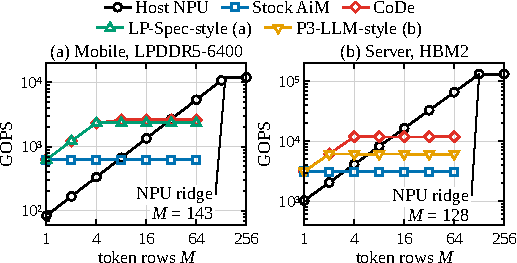
\includegraphics[width=\columnwidth]{figs/fig_roofline.pdf}
  \caption{Skinny-GEMM throughput against the number of token rows $M$: (a)~mobile platform; (b)~edge server.}
  \label{fig:roofline}
\end{figure}

\section{Background}
\label{sec:bg}

\subsection{Skinny GEMM in LLM Decoding}
\label{sec:bg:skinny}

% P:bg-skinny-range
A linear layer computes $Y = X W$ with a weight matrix $W$ of $K \times N$ and $M$ token rows in $X$. Plain decoding
($M = 1$) computes a GEMV. We call the layer a \emph{skinny GEMM} when $M \ll K, N$; this paper takes $2 \le M \le 32$
with $K$ and $N$ in the thousands, inside the bound $M \ll 64$ that FlashDecoding++~\cite{flashdecodingpp} reports for
decode GEMMs. A speculative decoder~\cite{leviathan2023} drafts tokens cheaply and verifies the $M$ drafted tokens in one
pass of the target model, as a chain or as a token tree~\cite{eagle2}; a batched decoder serves $M$ requests per step.
Published mobile decoders verify 2--8 drafted tokens padded to at most 32~\cite{sdnpu}, 1--32 on LPDDR-PIM~\cite{lpspec}
and token trees of 4--64~\cite{lever}, and edge-server batches hold 1--8 requests~\cite{p3llm}. Token trees for
datacenter GPUs (48--60~\cite{eagle2}, 64~\cite{medusa}, 64--128~\cite{sequoia}) and latency-capped datacenter batches
(16--27~\cite{attacc}) reach past that range, and there the GEMM moves to the host (Section~\ref{sec:bg:roofline}). This
paper targets verification on the mobile platform ($M = 2$--32~\cite{sdnpu,lpspec}) and batches on the edge server
($M = 2$--8~\cite{p3llm}).

\subsection{DRAM and AiM-Style PIM}
\label{sec:bg:pim}

% P:bg-dram-channel
A DRAM channel holds 16 banks in four bank groups (Fig.~\ref{fig:dram_pim}a). An activation opens one row of a bank,
2\,KB on LPDDR5~\cite{jedeclpddr5} (Table~\ref{tab:params}), into its sense amplifiers, and each column command moves
one 32\,B column of that row. Column commands may
issue every \tccds{} to different bank groups and every \tccdl{} to the same bank group, as the three reads of
Fig.~\ref{fig:dram_pim}b do; \tccdl{} is twice \tccds{} on LPDDR5~\cite{ramulator2} and on HBM~\cite{p3llm}.

% P:bg-aim-pu
AiM-style PIM adds a processing unit (PU) beside each bank (beside each pair of banks in HBM2) and a global buffer (GB),
shared by all PUs, that holds the input vector~\cite{aimjssc,hbmpim}; Fig.~\ref{fig:dram_pim}a enlarges one bank with
its PU. Commercial PIM ships the same per-bank layout, in HBM-PIM~\cite{hbmpim} and in Samsung's
LPDDR5X-PIM~\cite{lp5xpim}. An all-bank MAC command reads one column from every open bank at once and starts one MAC
beat in each PU; on the mobile platform, one beat is 32 INT8 multiplies of the column against 32 GB elements,
accumulated into the PU's output register. The all-bank command repeats every \tccdl~\cite{hbmpim}, the spacing of the
MAC commands in Fig.~\ref{fig:dram_pim}b. This column period \tcol spans $D = 4$ cycles \tck of the command clock CK on
both platforms (Table~\ref{tab:params}). We call $D$, the number of CK cycles in one column period, the \emph{depth};
\tcol equals $D \times \tck$.

% P:bg-mac-sequence
MAC commands need non-MAC commands before and after them (Fig.~\ref{fig:dram_pim}c). The all-bank MAC command is the
only MAC command; every other command is a non-MAC command. In the AiM command set~\cite{aimjssc}, as our simulator
issues it (Section~\ref{sec:method}), the non-MAC commands follow a fixed order: WRGB writes one token's input chunk into the GB once, and the MAC commands of every row that multiplies that chunk
read it from the GB. WRMAC16 sets the output registers to the bias. A mode switch (TMOD) moves the controller from
register commands to MAC commands, and PREA and ACT16 close the previous row and open the next one in all banks. After
the MAC commands, a second TMOD returns the controller to register commands, and RDMAC16 drains each token's sums.

% P:bg-row-sweep
A \emph{row sweep} streams $c$ all-bank MAC commands over one open row, one command per column, between these non-MAC
commands (Fig.~\ref{fig:dram_pim}c). The count $c$ is the row size over the column size: on the mobile platform,
$c = 2\,\text{KB} / 32\,\text{B} = 64$. An HBM2 row holds 1\,KB~\cite{jedechbm2}, so the edge server's row sweep covers
two rows opened in turn, 64 columns as well (Table~\ref{tab:params}). A row sweep serves the $A$ tokens whose inputs the GB
holds, and stock AiM's row sweep serves one ($A = 1$).

\section{Motivation}
\label{sec:motiv}

\subsection{PIM--Host Crossover}
\label{sec:bg:roofline}

% P:mot-roofline-setup
Fig.~\ref{fig:roofline} plots skinny-GEMM throughput against $M$ in the roofline form~\cite{roofline} for the host
NPU's roof and for simulated PIM GEMMs of stock AiM and each platform's rival. Each PIM curve is the geometric mean over
the FC shapes of the platform's models, and Fig.~\ref{fig:roofline} and the later throughput figures plot $M = 2^k$.
The mobile NPU is the Snapdragon 8 Gen 3's~\cite{sd8g3}, which reaches 56\,GB/s~\cite{powerinfer2} of its own
68\,GB/s pins~\cite{heterollm}; applied to the 51.2\,GB/s pins of x64 LPDDR5-6400, that fraction gives the NPU
42\,GB/s\ASSUMPTION. The edge-server NPU is P3-LLM's~\cite{p3llm}. Throughput numbers in this section are modelled on
the mobile platform and the edge server of Table~\ref{tab:params}, which Section~\ref{sec:method} details.

% P:mot-host-roof
\paragraph{Host roof in the skinny range}
The host stays memory-bound across the whole skinny range. The Snapdragon 8 Gen 3 NPU reaches its compute
roof only at $M \approx 143$, and P3-LLM's~\cite{p3llm} NPU reaches its roof at $M = 128$ (Fig.~\ref{fig:roofline}a,
b). Each NPU's ridge lies far above $M = 32$, so the host's roof rises linearly with $M$ across the skinny
range.

% P:mot-stock-crossover
\paragraph{Stock-PIM crossover}
Stock PIM beats the host only for the first few token rows. At $M = 1$ every PIM ceiling starts 9.75$\times$ above the
mobile NPU's roof and 4$\times$ above the edge-server NPU's roof. Stock AiM's ceiling is flat from $M = 1$, however,
because stock AiM repeats the GEMV once per token row, so its GEMM time grows in proportion to $M$. The rising host roof overtakes that ceiling, and stock
AiM wins a whole decode step only up to $M = 6$ on the mobile platform and $M = 2$--3 on the edge server, below most of
the published values of $M$ (Section~\ref{sec:bg:skinny}).

% P:mot-gemv-only
\paragraph{GEMV-only use of PIM}
Stock PIM is a GEMV engine, and published systems keep PIM for GEMVs and send the GEMMs to the host, even though the
host runs every skinny GEMM on its memory roof. AttAcc~\cite{attacc} runs batched FC layers on the xPU and attention on
PIM. NeuPIMs~\cite{neupims} maps the GEMMs to the NPU because PIM ``lacks the computational power to handle GEMM
effectively.'' IANUS~\cite{ianus} chooses NPU or PIM per FC layer. P3-LLM~\cite{p3llm} offloads its linear layers to
the NPU from batch 8, where its PIM becomes compute-bound.

% P:mot-a-summary
Skinny GEMMs are memory-bound on the host and thus belong on PIM, which reads the weights inside the DRAM, yet stock
PIM's GEMM throughput stays flat at its GEMV ceiling. Section~\ref{sec:bg:cmd} splits a stock GEMM's time to locate the
cause.

\subsection{Two Root Causes of Stock PIM Inefficiency}
\label{sec:bg:cmd}

% P:mot-breakdown-setup
Fig.~\ref{fig:breakdown} splits stock AiM's GEMM time into six components for one tile and for the query projection
layer (q\_proj) of Llama-2-7B on the mobile platform and of Llama-3.1-8B on the edge server; each bar is normalised to
its GEMM time, which is printed at the bar's end. The one tile's weights fill one row sweep in each bank and its inputs
fill one GB chunk ($K \times N$ of $2048 \times 64$ on the mobile platform and $4096 \times 256$ on the edge server),
so the one tile shows the costs of one row sweep. The q\_proj kernel, attention's $4096 \times 4096$ query projection,
shows a whole layer. Both kernels run at $M = 8$ on one channel. The mobile platform places an INT8 PU beside each
LPDDR5-6400 bank, and the edge server places a W4A8 PU beside each pair of HBM2 banks (Table~\ref{tab:params}). Each
platform computes at the precision of the prior PIM design that targets it, LP-Spec~\cite{lpspec} on the mobile platform
and P3-LLM~\cite{p3llm} on the edge server. The six
components form two groups: the time in non-MAC commands (row switch, token load, token drain and refresh) and the
time in MAC slots, which hold useful and idle beats. A MAC slot is the time \tslot that one all-bank MAC command
occupies; on the mobile platform a MAC slot spans one column period (Fig.~\ref{fig:dram_pim}b). Useful MAC work fills
at most a fifth of a stock GEMM's time: across the four bars, useful beats take 14.1--19.1\,\% of the time. Two root
causes take the rest: non-MAC commands between the MAC slots, 23.4--43.7\,\% of the time, and idle beats even inside
the MAC slots, 42.2--57.4\,\%.

% stock time-breakdown figure (cited first in III-B's first paragraph); generated by
% scripts/make_fig_breakdown.py (evaluation/dac_2x2 Sec. 2j, figures/tab_umac_kernel_stock.csv)
\begin{figure}[t]
  \centering
  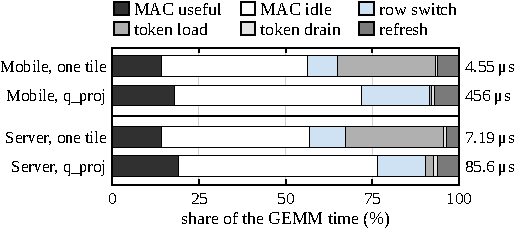
\includegraphics[width=\columnwidth]{figs/fig_breakdown.pdf}
  \caption{Stock AiM's GEMM time by component.}
  \label{fig:breakdown}
\end{figure}

% P:mot-nonmac-classes
\paragraph{Non-MAC commands}
Non-MAC commands (Section~\ref{sec:bg:pim}) stall every PU: no PU starts a MAC while they run. The four non-MAC
segments of Fig.~\ref{fig:breakdown}, row switch, token load, token drain and refresh, form three classes. The
\emph{row-switch commands}, the two TMODs, the PREA and ACT16 pair of each row opened and the WRMAC16, cost the
\emph{row-switch overhead} \trow once per row sweep. The \emph{token load/drain commands}, each token's share of WRGB
(token load) and its RDMAC16 (token drain), cost \ttok once per token. Refresh, the third class, blocks every command
for $t_\mathrm{RFCab}$ once per $t_\mathrm{REFI}$ (Table~\ref{tab:params}). With one token per stock row sweep, a GEMM
pays a row's row-switch commands $M$ times, where a GEMV pays them once.

% P:mot-rowswitch-cost
Row-switch commands are the largest class of non-MAC commands. In Fig.~\ref{fig:breakdown} the row-switch segment
takes 19.5\,\% of q\_proj's time on the mobile platform, more than the useful beats' 18.0\,\%, and 13.8\,\% on the edge
server. The two TMODs (8.1\,\%) and the ACT16 pair (8.5\,\%, timed by a simulator preset) take most of the mobile row
switch. The other two classes take less of q\_proj's time. Token load and token drain take at most 2.4\,\% and
1.0\,\%, because one GB fill serves all 64 row sweeps (mobile) or 16 (edge server) over its $K$ chunk, and refresh
takes 7.1\,\% on the mobile platform and 6.2\,\% on the edge server. On the edge server, the non-MAC commands together
take 23.4\,\%, more than the useful beats' 19.1\,\%.

% P:mot-sweep-factor
We define the share of the GEMM time that the MAC slots get as the \emph{sweep factor} \fMAC. For a row sweep of
$c$ MAC slots that serves $A$ tokens, the row-switch overhead, the token load/drain and refresh set \fMAC:
\begin{equation}
  \fMAC = \frac{(1 - \rho)\, c\, \tslot}{c\, \tslot + \trow + A\, \ttok}, \label{eq:fmac}
\end{equation}
where $\rho$ is the share of time that refresh takes. Fitted on stock AiM at $M = 1$ on the mobile platform, \trow
is 87.73\,ns, \ttok is 4.26\,ns and $\rho$ is 0.070, so stock AiM's MAC slots fill $\fMAC = 0.717$ of a decoder layer's
time.

% P:mot-idle-beats
\paragraph{Idle beats}
An idle beat is a CK cycle in which a PU has nothing to compute. A column period holds $D = 4$ such cycles, or beats
(Section~\ref{sec:bg:pim}), and a beat is useful when it computes a token's MAC. Stock AiM's MAC slot serves one token,
so one beat of each column period is useful and three are idle (Fig.~\ref{fig:dram_pim}b). The \emph{slot factor},
the useful share of a MAC slot, is $\UMAC = A \times b \times \tck / \tslot$, where $b$ is the number of beats per
token: $b = 1$ on the mobile platform, and $b = 2$ on the edge server, where each MAC command feeds a PU from its two
banks. Stock AiM's \UMAC is therefore 1/4. The idle segment is the largest of every bar in Fig.~\ref{fig:breakdown},
53.9\,\% of q\_proj's time on the mobile platform and 57.4\,\% on the edge server, three times the useful beats.

% P:mot-idle-cause
Idle beats arise because the column command, not the PU, paces every stock MAC: a MAC starts only when a column command
delivers its weights. HBM-PIM~\cite{hbmpim} executes one instruction per column command, and AiM~\cite{aimjssc} clocks
its PU at its interface's $t_\mathrm{CCD}$. Each column command reads one column, and DRAM timing lets the next column
command follow only after \tccds{} or \tccdl. Command pacing suits a GEMV, the target of these
PUs~\cite{aimjssc,p3llm}: in a GEMV each weight column meets one input vector, so one beat per column is enough.
Replacing stock AiM's PU, which runs one beat per column period, with a PU four times faster, clocked at CK, leaves
every stock GEMM at the same number of cycles.

% P:mot-utilization
The two losses multiply. The useful-MAC utilization $U$ is the MAC-useful share of each bar in
Fig.~\ref{fig:breakdown} and equals $W \times \tck / T_\mathrm{GEMM}$, where $W$ is the number of useful beats per PU
and $T_\mathrm{GEMM}$ is the GEMM time; $U$ thus measures a design against a PU that runs one useful beat per CK cycle. $U$ is the product
of the slot factor and the sweep factor, $U = \UMAC \times \fMAC$.
% useful-MAC table (cited first in III-B's closing paragraph): defined inside that paragraph so that it lands at the top
% of the column that cites it; generated by scripts/make_tables.py (simulated values, evaluation/dac_2x2 Sec. 2h)
\begin{table}[t]
  \caption{Useful-MAC utilization on the mobile platform.}
  \label{tab:umac}
  \centering
  \footnotesize
  \setlength{\tabcolsep}{3pt}
  % generated by scripts/make_tables.py from evaluation/dac_2x2/figures/tab_umac_paper.csv (umacp ids, simulated columns, M = 8); do not edit
\begin{tabular}{@{}lcccccc@{}}
\toprule
Design & $A$ & \tslot & \UMAC & \fMAC & $U$ & Non-MAC \\
 & & ns & & & & ns/token \\
\midrule
Stock AiM & 1 & 5 & 0.25 & 0.717 & 0.179 & 123.39 \\
P3-LLM-style & 2 & 5 & 0.50 & 0.709 & 0.355 & 63.94 \\
LP-Spec-style (4 ALUs) & 4 & 5 & 1.00 & 0.694 & 0.694 & 34.41 \\
\textbf{CoDe} ($V = 8$) & 8 & 10 & 1.00 & 0.779 & 0.779 & 22.15 \\
\bottomrule
\end{tabular}

\end{table}
Stock AiM's $U$ is $1/4 \times 0.717 = 0.179$ on the mobile platform (Table~\ref{tab:umac}) and 0.193 on the edge
server. Section~\ref{sec:bg:walls} examines how prior PIM designs answer each root cause.

\subsection{GEMM Support in Prior PIM}
\label{sec:bg:walls}

% P:mot-prior-families
Prior PIM designs fill the idle beats in two families, with more multipliers or with more commands
(Fig.~\ref{fig:timeline}). Fig.~\ref{fig:timeline} follows one weight column through eight tokens in stock AiM and in
one design of each family, LP-Spec~\cite{lpspec} for more multipliers and P3-LLM~\cite{p3llm} for more commands; the
next paragraphs take the two families in turn.

% P:mot-wider-pu
\paragraph{Wider-PU family}
Wider-PU designs trade area for MAC throughput: they fill the idle beats with more multipliers per PU.
LP-Spec~\cite{lpspec} builds its matrix unit from four 32-wide INT8 ALUs, clocks the ALUs at one MAC step per column
period, and shares one unit between two banks; we model one such unit per bank (Table~\ref{tab:params}). One column
command feeds the four ALUs with four tokens, one MAC step each. Fig.~\ref{fig:timeline} counts one bank's time in
column periods $T$ of $D = 4$ beats: where stock AiM spends 8 column periods, 8 commands and 8 reads on the 8 tokens,
the four ALUs need 2 of each, on four times the stock multipliers. The 4$\times$ ceiling moves the crossover of this
per-bank design with the host to $M = 20$--24 on the mobile platform (Fig.~\ref{fig:roofline}a).
PAPI~\cite{papi} places four processing units in each bank, and StepStone~\cite{stepstone} places SIMD units at the
bank groups or beside the devices of a memory module. Duplex~\cite{duplex} and H$^2$-LLM~\cite{h2llm} build their
multipliers on a logic die under the DRAM, and MoNDE~\cite{monde} builds them into a memory-side controller. We take
LP-Spec~\cite{lpspec} as the representative of the wider-PU family and model it as an \textbf{LP-Spec-style} design,
the rival on the mobile platform (Section~\ref{sec:eval:phone}). LP-Spec-style's slot serves four tokens, so
LP-Spec-style reaches $\UMAC = 1$ (Table~\ref{tab:umac}) only by quadrupling the multipliers: per multiplier its $U$
is 0.173--0.174 on the mobile platform and 0.185 on the edge server, below stock AiM's.

% timeline figure (cited first in III-C's opener; defined after mot-wider-pu so that it lands on the next page, not
% under Table I): column-width schematic; generated by scripts/make_fig_timeline.py
\begin{figure}[t]
  \centering
  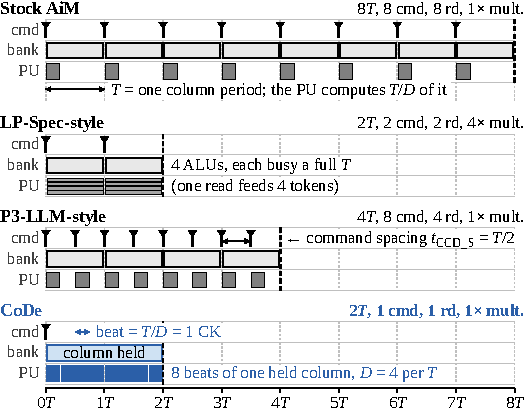
\includegraphics[width=\columnwidth]{figs/fig_timeline.pdf}
  \caption{One weight column of one bank in four designs; lanes show DRAM commands (cmd), column reads (bank) and MAC
  beats (PU).}
  \label{fig:timeline}
\end{figure}

% P:mot-logic-cost
\paragraph{Cost of logic in a DRAM die}
Logic in a DRAM die costs area: UPMEM~\cite{devaux} reports that a DRAM process builds logic 10$\times$ less dense
than an ASIC process and routes the logic in three metal layers instead of ten or more. In GDDR6-AiM~\cite{aimjssc} silicon, one PU occupies
0.19\,mm$^2$. Samsung's HBM-PIM~\cite{hbmpim} halves its DRAM sub-arrays to make room for its PUs and so gives up 50\,\% of
the die's memory capacity. By LP-Spec's~\cite{lpspec} own estimate its compute units and buffers take
16.92\,\% of a 16\,Gb LPDDR5 die, against 20--25\,\% of the chip for all of AiM's~\cite{aimjssc} compute circuits.
Four times the multipliers per bank therefore cost capacity, and per unit of logic area the wider-PU family keeps
only part of its 4$\times$ ceiling: LP-Spec-style's ceiling per logic mm$^2$ is 314\,GOPS on the mobile platform and
697 on the edge server, against stock AiM's 216 and 492.

% P:mot-faster-pu
\paragraph{Faster-PU family}
Faster-PU designs speed up the PU but still start every MAC with a command, so DRAM command timing, not the PU clock,
caps them at two beats per column read. P3-LLM~\cite{p3llm} keeps the weight of a column read latched in its PU,
issues one further command per token and clocks its PU at one beat per HBM2 \tccds{} (Table~\ref{tab:params}). Each
MAC thus still waits for its own command, as in stock AiM and LP-Spec-style (Fig.~\ref{fig:timeline}). Commands issue
only every \tccds, ``typically a half of \tccdl{}''~\cite{p3llm}, while the all-bank column runs at
\tccdl~\cite{hbmpim}, so at most two tokens share a read: the 8 tokens take 4 column periods, 8 commands and 4 reads.
On every memory family whose \tccdl{} is twice \tccds{}, the faster-PU family's \UMAC therefore stops at 1/2 however
fast its PU runs. The 2$\times$ ceiling moves the crossover of this design with the host to $M = 4$--6 on the edge
server (Fig.~\ref{fig:roofline}b). P3-LLM~\cite{p3llm} is the only design that applies a faster PU to $M > 1$, so we
take P3-LLM as the representative of the faster-PU family and model it as a \textbf{P3-LLM-style} design, the rival on
the edge server (Section~\ref{sec:eval:server}). With the stock multiplier count, P3-LLM-style's ceiling per logic
mm$^2$, 390\,GOPS on the mobile platform and 830 on the edge server, lies above LP-Spec-style's.

% P:mot-other-pim
The remaining LLM PIM designs fall outside the wider-PU and faster-PU families. GEMV-only designs serve one input
vector per weight read~\cite{newton,cent,pimgpt}, lookup-table designs replace multiplications with table
lookups~\cite{localut,pimpal,pimdl}, and scheduling and dataflow designs reorganize the work around the
PU~\cite{pimba,paise,splitsync,dots,pimphony}. Three designs, the closest prior art, run several MAC beats per column
read, yet each design holds one input vector ($M = 1$): SAL-PIM~\cite{salpim} clocks its MAC units at twice the column
rate, the Precision-Flexible PU~\cite{pfpu} runs four phases per column interval on packed low-bit operands, and
CD-PIM~\cite{cdpim} runs two compute units per bank at twice the internal clock. CD-PIM~\cite{cdpim} leaves the GEMM to
the host processor, and the extra beats of all three designs work on the same vector. Across the two families and
these three designs, a column read feeds several tokens only through added multipliers or added commands, and a row
sweep serves only the tokens of one MAC slot.

\subsection{The Opportunity: DRAM Timing Bounds Access, Not MACs}
\label{sec:bg:depth}

% P:mot-depth
DRAM timing bounds how often a column is read, not how many MACs may consume it. The PU takes its operands from the I/O sense amplifiers at the bank's I/O
boundary~\cite{hbmpim}, so a column the PU has latched stays usable after its command: P3-LLM~\cite{p3llm} reuses a
latched column for two tokens at unchanged cell-access and column-decoder power, the majority of PIM power. The column
period thus sets how often weights arrive at a PU, and the PU clock sets how often the PU computes on them, so a PU
clocked at CK can spend all $D$ beats of a column period on one latched column, as long as its MACs do not wait for
per-token commands.

% P:mot-pu-clock-precedent
A PU clocked at CK has precedent in DRAM silicon and in a PIM design for HBM2. HBM2's DRAM core runs at a quarter of
the 1.0--1.2\,GHz bus clock, and Samsung's HBM-PIM~\cite{hbmpim} sets its FP16 PU to the core frequency,
250--300\,MHz, in a 20\,nm DRAM process. Logic in later DRAM processes runs faster: UPMEM's processor~\cite{devaux}
is designed to execute 32-bit integer instructions at 500\,MHz in a 2x-nm DRAM process, a deployed UPMEM system
runs the processor at 350\,MHz~\cite{prim}, and GDDR6-AiM~\cite{aimjssc} runs BF16
multipliers and adder trees at 1\,GHz in a 1y-nm DRAM process. The 1y-nm process also builds HBM: Samsung's
HBM2E~\cite{flashbolt} stacks eight 1y-nm DRAM dies. The Precision-Flexible PU~\cite{pfpu} clocks an HBM-PIM-style
PU at CK on HBM2 and splits each 4-\tck column interval into four phases. DRAM periphery has gained logic-process
features: Samsung, SK hynix and Micron build periphery transistors with high-k metal gates~\cite{tiroadmap}, and
1a-nm dies route in five to six metal layers~\cite{tid1a16,tid1a24}.

% P:mot-two-levers
A PU at CK thus fits in a DRAM die, and the wider-PU family shows how much logic area a PIM die already gives to
filling idle beats. We therefore keep the stock multipliers, run them at CK within that area, and answer each root
cause of Section~\ref{sec:bg:cmd} with one lever. \emph{Row reuse} (Section~\ref{sec:design:reuse}) lets the $V$
tokens of a tile share one row sweep and pay its row-switch commands once, and answers the non-MAC commands by cutting
their time per token. \emph{Beat filling} (Section~\ref{sec:design:beat}) uses all $D$ beats of a column period
(Fig.~\ref{fig:dram_pim}b) without adding multipliers and answers the idle beats.

\section{CoDe Design}
\label{sec:design}

% float placed early (cited first in IV-A): column-width schematic, figs/src/fig_tile.html (hand-maintained)
\begin{figure}[t]
  \centering
  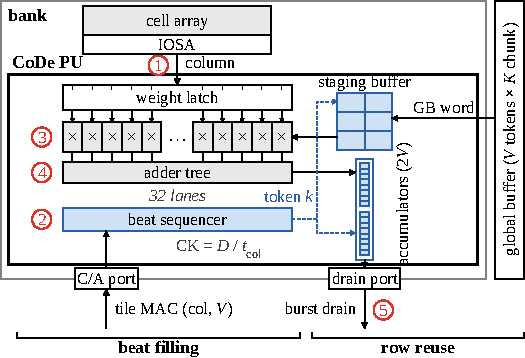
\includegraphics[width=\columnwidth]{figs/fig_tile.pdf}
  \caption{The CoDe PU inside its bank; tint marks the structures CoDe adds or sizes by $V$.}
  \label{fig:tile}
\end{figure}

\subsection{Overview: One Command, Many MAC Beats}
\label{sec:design:overview}

% P:des-tile-mac-overview
CoDe (Command-Decoupled PIM) issues one MAC command per weight column for a tile of $V$ token vectors of a skinny
GEMM, and this single \emph{tile MAC} command carries CoDe's two levers: row reuse (Section~\ref{sec:design:reuse})
and beat filling (Section~\ref{sec:design:beat}). Every command still obeys every DRAM timing parameter: activations,
column reads and refreshes issue exactly as in stock AiM, and only the MAC beats leave the command stream. Both levers
come from the tile, and the tile comes from the global buffer, which CoDe extends from stock AiM's one input vector to
the input vectors of $V$ tokens (Fig.~\ref{fig:tile}, Section~\ref{sec:design:pu}): sharing a row sweep needs $V$
tokens' inputs beside the PU, and filling $D$ beats needs at least $D$ tokens per command. Fig.~\ref{fig:tile} groups
the PU's structures by lever: the staging buffer, the accumulator file and the burst drain carry row reuse, and the
weight latch and the beat sequencer carry beat filling. With both levers, CoDe's useful-MAC utilization $U$ reaches
0.779 on the mobile platform, against stock AiM's 0.179 (Table~\ref{tab:umac}).

% float placed after IV-A (cited first in IV-B); generated by scripts/make_fig_mapping.py (evaluation/dac_2x2 Sec. 2j,
% raw/utrace_run_{stock,core8}.csv), which asserts every number IV-B and IV-C print from the trace
\begin{figure}[t]
  \centering
  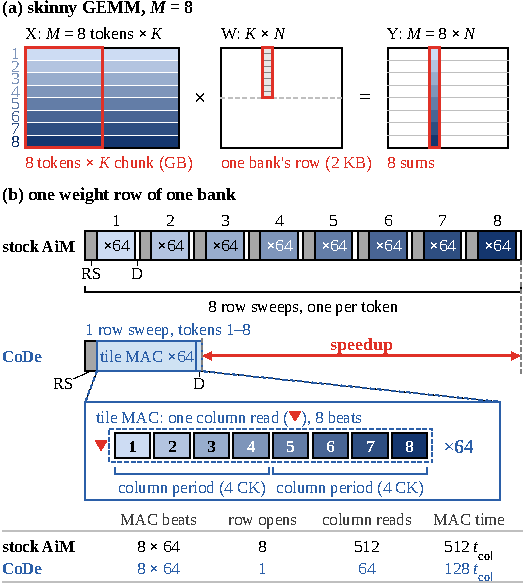
\includegraphics[width=\columnwidth]{figs/fig_mapping.pdf}
  \caption{A skinny GEMM at $M = 8$: (a)~one bank's work per row sweep; (b)~one weight row, stock AiM and CoDe, one
  tile MAC enlarged. RS = row switch; D = drain.}
  \label{fig:mapping}
\end{figure}

\subsection{Row Reuse}
\label{sec:design:reuse}

% P:des-row-reuse
Row reuse answers the non-MAC commands of Section~\ref{sec:bg:cmd}, whose row-switch commands stock AiM pays once per
token. Row reuse lets the $V$ tokens of a tile share one row sweep: the tile MACs sweep the open row's columns once for
all $V$ tokens, so the row-switch commands are paid once per $V$ tokens. Fig.~\ref{fig:mapping}a draws the tile in
GEMM terms at $M = V = 8$: the GB holds the eight tokens' inputs for one chunk of $K$, one bank's open 2\,KB row holds
one output's weights over that chunk, and the tile produces that output's eight sums. In Fig.~\ref{fig:mapping}b,
stock AiM sweeps the weight row once per token and pays a row switch and a drain in each of its eight sweeps, whereas
CoDe pays one row switch for the tile; the row opens fall from eight to one and the column reads from 512 to 64,
because the tile reads each weight from the array once. With $A$ tokens per row sweep, a token pays
$\trow / A + \ttok$ of non-MAC commands per row sweep, plus its share of refresh. The token load/drain commands stay
per token: WRGB writes each token's input chunk into the GB, and the burst drain reads each token's sums once per row
sweep. Row reuse needs the $V$ tokens' inputs next to the PU for the whole row sweep and $V$ partial sums per tile; the
global buffer, the staging buffer and the accumulator file hold them (Section~\ref{sec:design:pu}). The two families
of Section~\ref{sec:bg:walls} tie the tokens of a row sweep to one MAC slot ($A = 2$ and 4 in Table~\ref{tab:umac}),
whereas CoDe sets them by $V$ and leaves the PU's lanes unchanged. The simulated non-MAC time per token thus falls
from stock AiM's 123.39\,ns to CoDe's 22.15\,ns at $V = 8$ on the mobile platform (Table~\ref{tab:umac}) and from
146.17 to 43.51\,ns at $V = 4$ on the edge server.

\subsection{Beat Filling}
\label{sec:design:beat}

% P:des-beat-decouple
Beat filling answers the idle beats of Section~\ref{sec:bg:cmd}, three of a stock MAC slot's four beats, by decoupling
the PU's MAC beats from the command stream. The PU runs its beats at its own clock, $f_\mathrm{PU} = D /
t_\mathrm{col}$, which equals CK on both platforms (Table~\ref{tab:params}), so the PU fits $D$ beats into each column
period whatever the command spacing. A tile MAC holds its column in the PU for $V/D$ column periods, and the next tile
MAC issues $V/D$ periods later. The enlarged tile MAC of Fig.~\ref{fig:mapping}b shows one tile of $V = 8$ tokens at
$D = 4$: one column read feeds eight beats, one per token and four per column period, and each beat adds into its
token's accumulator slot. The bank holds the column for $V/D = 2$ periods, the next tile MAC issues two periods later,
and the tile's partial sums leave in one burst drain after its last column. With $V = D$ the tile fills exactly one
column period, and the MAC commands follow the bank's column rate.

% P:des-beat-slot-factor
Beat filling raises the slot factor from stock AiM's 1/4 to 1, because every beat of a MAC slot computes for one token
of the tile. A PU with the stock multiplier count thus reaches the 4$\times$ ceiling that the wider-PU family reaches
with four times the multipliers. Against the faster-PU family, beat filling saves commands: per token and weight
column, CoDe issues $1/V$ MAC commands, against one for stock AiM and P3-LLM-style and $1/4$ for LP-Spec-style
(Fig.~\ref{fig:timeline}). In the table of Fig.~\ref{fig:mapping}b, the weight row's time in MAC slots falls from 512
to 128 column periods for the same $8 \times 64$ MAC beats. With both levers joined, the weight row takes 738.75\,ns
against stock AiM's 3,250\,ns, 4.40$\times$ shorter, the speedup gap of Fig.~\ref{fig:mapping}b.

\subsection{Tile MAC Command and PU Microarchitecture}
\label{sec:design:pu}

% P:des-command-set
\paragraph{Command set}
CoDe adds two commands to the all-bank interface of AiM-style PIM~\cite{aimjssc} and keeps every other command
(Table~\ref{tab:cmds}). The tile MAC (col, $V$) reads one column from every open bank with the stock MAC command's
timing and tells each PU to run $V$ beats on that column. The burst drain moves a tile's $V$ sums out of every PU in
one burst after the tile's last column. WRGB, TMOD, PREA, ACT16 and WRMAC16 keep their stock definitions, and of these
only the row-switch commands change their count per token.


% P:des-tile-mac-pu
\paragraph{Tile MAC in the PU}
Fig.~\ref{fig:tile} follows one tile MAC through the PU. The tile MAC latches the column that the bank delivers in the
weight latch (\ding{172}). The beat sequencer then steps a token index $k$ from 0 to $V-1$, one beat per CK cycle
(\ding{173}). Beat $k$ multiplies the latched weights by token $k$'s slice from the staging buffer in the lanes (\ding{174}), and the adder
tree adds the products into accumulator slot $k$ (\ding{175}). After the tile's last column, the burst drain moves the
$V$ sums out through the drain port (\ding{176}).

% P:des-storage
\paragraph{Storage}
The global buffer holds the tile's $V$ tokens for one chunk of $K$. On the mobile platform a $K$ chunk holds 2,048 INT8
inputs, 2\,KB per token, so the GB of an eight-token tile holds 16\,KB (Table~\ref{tab:params}); one WRGB burst of 512
writes of 32\,B fills it. The staging buffer next to the lanes is a three-entry queue of 512-bit GB words on the mobile platform, each word
packing two tokens' slices, and a register of $V$ slices on HBM2. The accumulator file holds two sets of $V$ slots per bank, so
one tile's sums drain from one set while the next tile accumulates into the other; an HBM2 PU, which serves two banks,
holds four sets (Table~\ref{tab:params}).

% P:des-tile-size
\paragraph{Tile size}
The tile size $V$ sizes CoDe's storage: the GB holds $V$ tokens' $K$ chunks, the HBM2 staging register holds $V$
slices, and the accumulator file holds two sets of $V$ slots per bank. The lanes, the weight latch, the beat sequencer and the
mobile staging queue keep their size at any $V$. Below $V = D$ the column period paces the PU and beats idle; from
$V = D$ every beat computes, and a larger $V$ cuts only the row-switch term of a token's non-MAC time per row sweep,
about $\trow / V + \ttok$. A weight row takes $\lceil M/V \rceil$ row sweeps, so a last sweep with fewer than $V$
tokens, or any $V > M$, leaves slots idle, and $V$ is sized for the range of $M$ a platform serves. CoDe sets
$V = 2D = 8$ on the mobile platform and $V = D = 4$ on HBM2, where each token needs twice the storage, a 4\,KB $K$
chunk and a 512-bit slice, and one PU serves two banks, so an added slot costs a larger share of the logic
(Section~\ref{sec:eval:ablation}).

% command table (cited first in IV-D): defined in IV-D's right-hand column, so it renders at that column's
% top, opposite Fig. tile; generated by scripts/make_fig_mapping.py
\begin{table}[t]
  \caption{CoDe's commands, counted per token against stock AiM.}
  \label{tab:cmds}
  \centering
  \footnotesize
  \setlength{\tabcolsep}{2.5pt}
  % generated by scripts/make_fig_mapping.py (counts checked on the V = 8 trace, evaluation/dac_2x2 Sec. 2j); do not edit
\begin{tabular}{@{}l>{\raggedright\arraybackslash}p{3.2cm}lcc@{}}
\toprule
Command & Action & Unit & CoDe & Stock \\
\midrule
\emph{tile MAC} (col, $V$) & One column read at the stock MAC timing; $V$ beats on it & column & $1/V$ & 1 \\
\emph{burst drain} & A tile's $V$ sums out in one burst & row sweep & 1 & 1 \\
row switch & TMOD$\times$2, PREA, ACT16 pair, WRMAC16; unchanged & row sweep & $1/V$ & 1 \\
WRGB & GB fill; unchanged & 32\,B of input & 1 & 1 \\
\bottomrule
\end{tabular}

\end{table}

% P:des-pu-clock
\paragraph{PU clock}
CoDe needs a PU clock above the column rate, not one equal to CK, and the tile keeps that clock within the reach of
the DRAM silicon of Section~\ref{sec:bg:depth}. Beat $k$ writes
accumulator slot $k$, so each slot takes one update per tile of $V \ge D$ beats, and the add loop of each slot spans a
column period or more. CoDe's lanes multiply integers, INT8 on the mobile platform and INT4\,$\times$\,INT8 on HBM2,
narrower operands than the BF16 of that section's 1\,GHz multipliers. Each added structure grows with $V$, not with
$D$: CoDe spends its area on storage and keeps the stock multiplier count (Section~\ref{sec:method}).

\subsection{Mapping Skinny GEMMs and Attention}
\label{sec:design:map}

% P:des-mapping
A $K \times N$ weight matrix maps as in stock AiM: the matrix's $N$ output rows spread over the banks, and each row's $K$ weights run along DRAM columns. CoDe cuts the $M$ token rows into tiles of $V$. For each tile the GB holds the tile's
activations for a chunk of $K$; every weight column of the chunk takes one tile MAC command, and the next tile repeats
the row sweep. A tile with fewer than $V$ tokens runs fewer beats on the same commands. Attention runs on the same path
with the KV cache as the weight matrix: $QK^\top$ streams the cached keys against the $M$ query rows, and $PV$ the
cached values against the $M$ rows of probabilities. Speculative decoding verifies $M$ drafted tokens against one
shared KV cache, so speculative-decoding attention is a skinny GEMM as well; a batch reads one cache per request, so batched attention
stays one GEMV per request. The host computes softmax, RoPE and normalisation between the PIM phases.

\section{Methodology}
\label{sec:method}
\label{sec:eval:method}% alias: the former Evaluation subsection

\subsection{Hardware Platforms}
The mobile platform pairs the Snapdragon 8 Gen 3~\cite{sd8g3} host and NPU with PIM on LP-Spec's~\cite{lpspec} x64
LPDDR5-6400 (4 dies $\times$ 16 banks, 409.6\,GB/s internal). The NPU computes at 12\,TOPS, its measured FP16 GEMM rate~\cite{hao2025}
used for INT8\ASSUMPTION, and reads the memory at 42\,GB/s (Section~\ref{sec:bg:roofline}). Each host visit costs
30\,\textmu s of NPU dispatch~\cite{npufaster}\ASSUMPTION; the host draws 2.285\,W while busy, the 8 Gen 3's~\cite{sd8g3}
decode power net of its DRAM~\cite{hao2025,heterollm,tman}\ASSUMPTION. The edge server pairs P3-LLM's~\cite{p3llm} NPU with one
HBM2 stack of 16 pseudo-channels (1,024\,GB/s internal); the NPU idles at 55\,W, the chip idle power of
TPUv4i~\cite{tpuv4i}, while the PIM works\ASSUMPTION.

\subsection{PIM Designs and Area}
Each substrate carries four designs, stock AiM~\cite{aimjssc}, P3-LLM-style, LP-Spec-style and CoDe, with one
controller and the same PU placement (Table~\ref{tab:params}). Every design computes at its rival's
precision: INT8 on the mobile platform, as LP-Spec~\cite{lpspec} does, and W4A8 with a 4-bit KV cache on HBM2, as
P3-LLM~\cite{p3llm} does, with every design's arithmetic priced as INT4\,$\times$\,INT8 integers\ASSUMPTION. On the
mobile platform CoDe's tile of $V = 8$ spans two column periods, so one MAC command serves eight tokens. On HBM2 each
token's staging slice is twice as large and every PU serves two banks, so CoDe uses $V = D = 4$
there; Section~\ref{sec:eval:ablation} sizes $V$ on both platforms. CoDe reaches LP-Spec-style's peak on
the mobile platform with 0.539$\times$ its logic area per die: arithmetic takes 0.73 of LP-Spec-style's logic and 0.34
of CoDe's, while storage, the staging queue, accumulator file and weight latch, takes 0.32 of CoDe's logic and 0.10
of LP-Spec-style's. On HBM2, CoDe's logic is 0.56$\times$ LP-Spec-style's and 1.33$\times$ P3-LLM-style's, an area
that buys twice P3-LLM-style's beats per column.

\subsection{Simulator and Models}
% figure* (Section VI-A): defined at V-C's start (page 8), so it renders at the top of the next page, where VI-A cites it
\begin{figure*}[t]
  \centering
  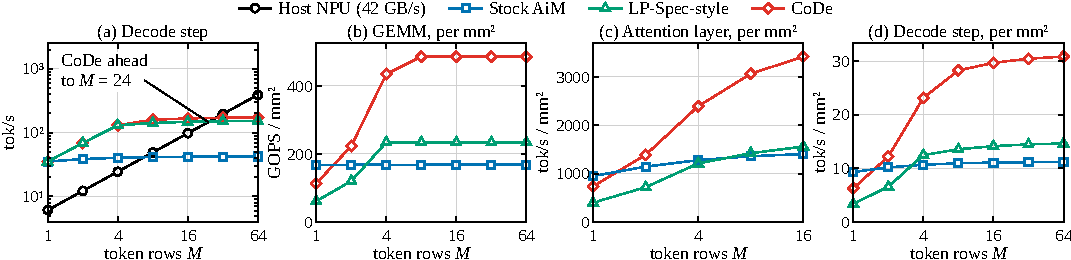
\includegraphics[width=\textwidth]{figs/fig_phone.pdf}
  \caption{Mobile platform: (a)~decode-step speed; (b)~GEMM, (c)~attention-layer and (d)~decode-step throughput per
  logic mm$^2$.}
  \label{fig:phone}
\end{figure*}

We extend the open-source trace-driven AiM simulator, built on Ramulator~2.0~\cite{ramulator2} and used by
CENT~\cite{cent}, with each design's commands and a PU model that holds a MAC command until the PU has finished the
beats of the previous command; every PIM kernel runs at cycle level. Our P3-LLM-style model reproduces
P3-LLM's~\cite{p3llm} own step gain of depth 2 over a depth-1 PIM: 1.78$\times$ at INT8 against the 1.6$\times$ P3-LLM
reports. On the mobile platform the simulator gives P3-LLM-style's per-token commands no separate C/A slot;
re-timed on the C/A bus, the commands lower P3-LLM-style's $U$ from 0.384 to 0.380, and on the edge server the
simulator times them. The mobile runs issue refreshes without their refresh cycle time, so refresh takes no share of
the mobile time ($\rho = 0$ in Section~\ref{sec:bg:cmd}). Area comes from synthesis of each PU's lanes and registers in a 45\,nm library, scaled to a 1z DRAM process by
the published area of AttAcc's~\cite{attacc} GEMV unit in that process; the GB is priced as DRAM-process
SRAM\ASSUMPTION. PU power and energy come from synthesis of each design's whole PU with Yosys and ABC~\cite{abc} on the
Nangate45 library, OpenROAD~\cite{openroad} placement and clock-tree synthesis, and OpenSTA power from a zero-delay
simulation with random operands. We scale the synthesised energy to the DRAM process so that an AiM-style bf16 PU from
the same flow spends the compute share of CENT's~\cite{cent} AiM MAC-command energy, and with the square of the voltage
to the 1.05\,V supply (VDD2H on LPDDR5); leakage scales the same way\ASSUMPTION. Peak power runs every PU at its full
MAC rate and includes leakage, GB reads and the column fetch, which adds 87.6\,mW per die on the mobile platform and
54.8\,mW per pseudo-channel on HBM2 to every design. Energy per token charges each issued MAC its PU's synthesised energy,
leakage over the step time, GB reads priced by SRAM size~\cite{horowitz}, and CENT's~\cite{cent} per-command DRAM
energies. In every design a PU's clock runs only on its MAC beats, so an idle PU cycle costs leakage
only\ASSUMPTION.

\subsection{Algorithms and Workloads}
The mobile platform runs speculative decoding of Llama-2-7B in INT8 with a 1.1B-parameter draft model or an EAGLE
head~\cite{eagle}: $M - 1$ drafted tokens and one verify pass of $M$ rows, acceptance rate 0.7 per token, context
$L = 128$--1024, and each design at its fastest $M$. GEMMs use six FC shapes of Llama-2-7B and Llama-3.2-1B, and attention layers use three head configurations at $L = 128$--4096. The edge server runs batched decoding of Llama-2-7B
and 13B, Llama-3.1-8B, Llama-3.2-3B and Mistral-7B at a 4K context, batch $M = 1$--64, one token per request per step.

\subsection{Metrics}
Speed is tokens per second, end to end or of one decode step; area efficiency is that throughput per mm$^2$ of PIM
logic, over all four dies or all 16 pseudo-channels; energy is system energy per token. On HBM2 one all-bank column counts as one command and as two half-column slots in the C-bus occupancy. Ranges on the mobile platform span every $M$ and $L$; ranges on the edge server are the minimum and maximum of per-$M$ geometric means over the five models.

\section{Evaluation}
\label{sec:eval}

% P:eval-modelled
All results are modelled, and ratios above 1 favour CoDe.

\subsection{GEMM Speed and Area Efficiency}
\label{sec:eval:gemm}

% P:eval-gemm-summary
CoDe matches LP-Spec-style's GEMM speed on about half its logic and outruns P3-LLM-style once a GEMM has more than two
token rows. Fig.~\ref{fig:gemm} plots each design's GEMM speed-up over stock AiM and its GEMM throughput per logic
mm$^2$ against $M$, with the NPU's GEMM speed as a line; each point is the geometric mean over the FC shapes of
Section~\ref{sec:method:work}.

% P:eval-gemm-speed
\paragraph{GEMM speed}
Up to $M = 2$ the column period paces every design: one column read serves every token, and P3-LLM-style,
LP-Spec-style and CoDe all run 1.96--1.97$\times$ faster than stock AiM at $M = 2$ (Fig.~\ref{fig:gemm}a). From
$M = 3$ P3-LLM-style needs a second pass for the tokens beyond its two per read, while CoDe fills up to four beats per
command: at $M = D = 4$ CoDe runs 3.74$\times$ stock AiM's speed on the mobile platform and 3.82$\times$ on the edge
server, against P3-LLM-style's 1.95$\times$. LP-Spec-style also fills four beats per column period, with four times
the multipliers, so its curve coincides with CoDe's up to $M = 4$, and at every $M$ on the edge server, where CoDe's
tile of $V = D = 4$ issues LP-Spec-style's command stream. On the mobile platform CoDe's eight-token tile also covers
$M = 5$--8 in one row sweep where LP-Spec-style needs a second pass, and CoDe runs 1.62$\times$ LP-Spec-style's speed
at $M = 5$.

% P:eval-gemm-per-mm2
\paragraph{GEMM throughput per logic mm$^2$}
Per logic mm$^2$, CoDe nearly doubles LP-Spec-style's GEMM throughput on both platforms. CoDe fills the same beats as
LP-Spec-style but spends its logic on storage rather than multipliers, so it reaches LP-Spec-style's speed with
0.539$\times$ its logic area on the mobile platform and 0.56$\times$ on the edge server
(Section~\ref{sec:method:designs}). CoDe therefore returns 1.86$\times$ LP-Spec-style's GEMM throughput per logic
mm$^2$ on the mobile platform up to $M = 4$ and 1.99--2.07$\times$ from $M = 8$, with a peak of 3.01$\times$ at
$M = 5$, where LP-Spec-style runs its second pass; on the edge server the ratio is 1.79$\times$ at every $M$
(Fig.~\ref{fig:gemm}b). Against P3-LLM-style, CoDe's speed outgrows its larger logic from $M = 3$: CoDe returns
1.43$\times$ P3-LLM-style's throughput per logic mm$^2$ at $M = 4$ and 1.53--1.59$\times$ from $M = 8$ on the mobile
platform, and 1.46--1.48$\times$ at $M = 3$--4 and from $M = 8$ on the edge server. Only at $M \le 2$, where CoDe's
third and fourth beats sit idle, does P3-LLM-style's smaller PU lead, with CoDe at 0.75$\times$.

% figure* (Section VI-B): placement checked on the float map after each build
\begin{figure*}[t]
  \centering
  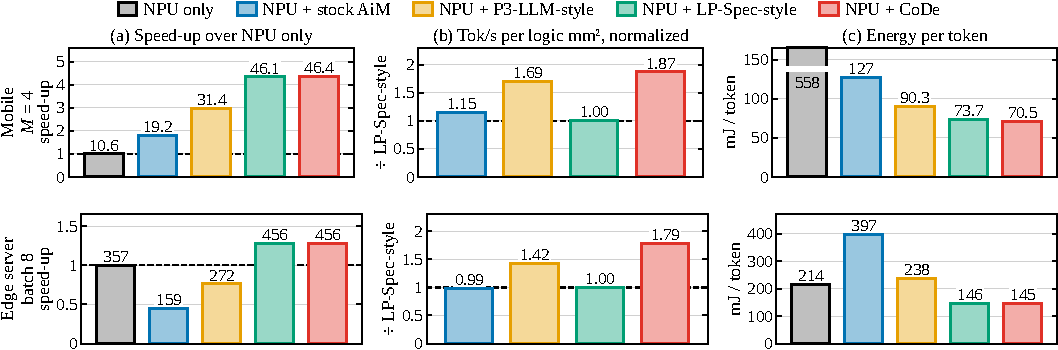
\includegraphics[width=\textwidth]{figs/fig_e2e.pdf}
  \caption{End-to-end decoding, mobile platform (top) and edge server (bottom): (a)~speed-up over NPU only, tokens/s
  on bars; (b)~tokens/s per logic mm$^2$; (c)~energy per token.}
  \label{fig:e2e}
\end{figure*}

\subsection{End-to-End Speedup}
\label{sec:eval:e2e}

% P:eval-e2e-phone
\paragraph{Mobile platform}
Fig.~\ref{fig:e2e} runs whole decoding on the five systems of Section~\ref{sec:method:work}: the speculative loop at
$M = 4$ on the mobile platform and a batch of 8 on the edge server. On the mobile platform CoDe and LP-Spec-style
decode fastest, 4.37$\times$ and 4.34$\times$ faster than NPU only, at 46.4 and 46.1 tokens/s
(Fig.~\ref{fig:e2e}a). P3-LLM-style reaches 2.96$\times$, because its two-token read needs two passes over the four
token rows, and stock AiM reaches 1.81$\times$. At each system's own best $M$ the order holds: CoDe reaches
47.1 tokens/s and LP-Spec-style 46.8 at $M = 3$, P3-LLM-style 43.8 and stock AiM 26.5 at $M = 2$, and NPU only 10.6
at $M = 4$. Past $M = 4$ CoDe's eight-token tile pulls ahead: CoDe's loop runs 1.31$\times$ faster than
LP-Spec-style's at $M = 5$ and 1.05--1.31$\times$ faster over $M = 5$--16.

% P:eval-e2e-server
\paragraph{Edge server}
On the edge server only CoDe and LP-Spec-style decode a batch of 8 faster than NPU only, both 1.28$\times$ at
456 tokens/s (Fig.~\ref{fig:e2e}a). Stock AiM runs at 0.45$\times$ and P3-LLM-style at 0.76$\times$ NPU only's speed,
so at the batch where P3-LLM~\cite{p3llm} moves its linear layers to the NPU, CoDe decodes 1.68$\times$ faster than
P3-LLM-style. On the geometric mean over the five models, NPU only overtakes CoDe from batch 16.

% P:eval-e2e-per-mm2
\paragraph{Throughput per logic mm$^2$}
At LP-Spec-style's decoding speed, CoDe nearly doubles LP-Spec-style's tokens per second per logic mm$^2$ on both
platforms. CoDe returns 1.87$\times$ LP-Spec-style's decoding throughput per logic mm$^2$ on the mobile platform and
1.79$\times$ on the edge server (Fig.~\ref{fig:e2e}b), because CoDe matches LP-Spec-style's speed on about half its
logic. Against P3-LLM-style, whose PU takes less logic than CoDe's, CoDe's speed lead more than repays the area:
CoDe returns 1.10$\times$ P3-LLM-style's decoding throughput per logic mm$^2$ on the mobile platform and 1.26$\times$ on the
edge server.

\subsection{Energy and Peak Power}
\label{sec:eval:energy}

% P:eval-energy
\paragraph{Energy per token}
CoDe spends the least energy per token of the five systems on both platforms. On the mobile platform the speculative
loop on CoDe spends 70.5\,mJ per token at $M = 4$, while NPU only spends 7.9$\times$, stock AiM 1.80$\times$,
P3-LLM-style 1.28$\times$ and LP-Spec-style 1.04$\times$ CoDe's energy (Fig.~\ref{fig:e2e}c). On the edge server,
with the NPU idling at 55\,W while the PIM works, NPU only spends 1.48$\times$ and P3-LLM-style 1.64$\times$ CoDe's
energy per token, and LP-Spec-style ties CoDe; with the idle NPU power-gated, P3-LLM-style still spends 1.46$\times$
CoDe's energy.

% P:eval-power
\paragraph{Peak power}
CoDe's faster PU clock keeps its peak power within a few percent of LP-Spec-style's, and each of its clock edges
draws less charge. With every PU at its full MAC rate, CoDe draws 1.04$\times$ LP-Spec-style's peak power per die on
the mobile platform and 1.03$\times$ per pseudo-channel on HBM2 (Table~\ref{tab:params}); stock AiM and P3-LLM-style
draw less because they run fewer MACs per column period. CoDe spreads the same MAC rate over four times as many clock
edges: its PUs switch 522\,pJ per die every 1.25\,ns against LP-Spec-style's 1,776\,pJ every 5\,ns, so each CoDe edge
draws 3.4$\times$ less charge, and 3.1$\times$ less on HBM2, which lowers the current step that the die's power grid
absorbs. Clock gates on CoDe's mostly idle accumulator slots and staging words would cut its peak power to
0.92$\times$ and 0.87$\times$ ungated LP-Spec-style's; every other number describes the ungated designs.

\subsection{Ablation Study}
\label{sec:eval:ablation}

% P:eval-gain-sources
\paragraph{Sources of CoDe's gain}
CoDe's gain over stock AiM has two sources, row reuse and beat filling, and each source is worth more once the other
is present. Table~\ref{tab:umac_src} adds the two sources with row reuse first for one decoder layer's weight GEMMs at $M = 8$, the layer of Table~\ref{tab:umac} on the mobile platform and
of Llama-3.1-8B on the edge server. The row-reuse-only design keeps the stock PU's pace of one beat per column
period and adds CoDe's storage and row sweeps of $V$ tokens; we simulate it as CoDe's trace at $D = 1$. Row reuse alone speeds
the layer up 1.24$\times$ on the mobile platform and 1.15$\times$ on the edge server, yet $U$ reaches only 0.223 and
0.222, because \UMAC stays at 1/4.
Beat filling, the command decoupling of Section~\ref{sec:design:beat}, then fills the idle beats and supplies the large step,
3.49$\times$ on the mobile platform and 3.33$\times$ on the edge server, while CoDe's \fMAC of 0.779 and 0.739 stays
near stock AiM's 0.717 and 0.771. In the other order, which we model as a quarter of stock AiM's MAC slots plus its non-MAC time per row sweep rather
than simulate, beat filling alone would cut \fMAC,
and with \UMAC at 1 also $U$, to 0.425 and 0.506, in steps of 2.37$\times$ then 1.83$\times$ on the mobile platform
and 2.62$\times$ then 1.46$\times$ on the edge server: the unchanged non-MAC commands would take more than half of the
shortened time on the mobile platform and about half on the edge server. Beat filling thus earns its full step only
once row reuse has removed most of the row-switch overhead per token.

% P:eval-vsweep-summary
\paragraph{Choice of tile size}
Throughput per logic mm$^2$ peaks at the tile size $V = D$ on both platforms, and the mobile platform's $V = 8$
bounds the per-mm$^2$ loss across the token rows of a decode step. Fig.~\ref{fig:vsweep}a sweeps $V$ from 1 to 64 for
q\_proj at $M = 64$ with the staging of Section~\ref{sec:design:pu}, which on the mobile platform is a register of
$V$ slices below $V = 8$; Fig.~\ref{fig:vsweep}b sets $V = 8$ against $V = 4$ for $M = 1$--16.

% P:eval-vsweep-gain
\paragraph{Gain by tile size}
Up to $V = D$ a larger tile fills idle beats; beyond $V = D$ it removes only row-switch commands. CoDe's q\_proj
speed-up over stock AiM rises from 1 at $V = 1$ to 3.86$\times$ on the mobile platform and 3.69$\times$ on HBM2 at
$V = D$, but only to 4.90$\times$ and 4.39$\times$ at $V = 64$. On the mobile platform, of the time that the step from
$V = 1$ to 2 saves, idle beats supply 72\,\%, row-switch commands 21\,\% and refresh 7\,\%. From $V = 4$ to 8 the
row-switch commands supply 91.6\,\% of the saving, and their share of the GEMM time falls from 18.9\,\% to 10.4\,\%;
token load stays at 20.5\,$\mu$s at every $V$.

% P:eval-vsweep-area
\paragraph{Area against speed}
Past $V = D$ CoDe's storage grows faster than its speed. Fig.~\ref{fig:vsweep}a normalises throughput per logic
mm$^2$ to stock AiM's, and both per-mm$^2$ curves peak at $V = D$, at 3.01$\times$ on the mobile platform and
2.34$\times$ on HBM2. From $V = 4$ to 8 the mobile
logic grows by 16\,\%, from 1.212 to 1.406\,mm$^2$ per die, and HBM2's by 40\,\%, from 0.821 to 1.153\,mm$^2$ per
pseudo-channel, so $V = 8$ breaks even per mm$^2$ only at 1.160$\times$ and 1.405$\times$ $V = 4$'s speed. At
$M = 64$, $V = 8$ runs 1.117$\times$ and 1.089$\times$ faster and keeps 96.3\,\% and 77.5\,\% of the peak.

% P:eval-vsweep-robust
\paragraph{Robustness across $M$}
Partial last row sweeps make $V = 8$ win per mm$^2$ on the mobile platform at $M = 5$--7, 9--10 and 13--15. At
$M = 5$, $V = 4$ runs two row sweeps of three and two tokens where $V = 8$ runs one, and $V = 8$'s verify step
returns 1.324$\times$ $V = 4$'s throughput per mm$^2$; up to $M = 4$ both tiles run one row sweep and $V = 8$ returns
0.862$\times$ (Fig.~\ref{fig:vsweep}b). HBM2's batched step never reaches the 1.405$\times$ break-even, and $V = 8$
peaks at 0.944$\times$ at $M = 5$. Against the best of $V = 2$, 4, 8 and 16 at each $M$ from 3 to 16, the mobile
$V = 4$'s worst per-mm$^2$ loss is 29.4\,\% on q\_proj and 24.5\,\% on the verify step, both at $M = 5$, while
$V = 8$'s is 13.8\,\%, its area premium at $M = 3$--4. On HBM2, $V = 4$ loses at most 11.7\,\% and $V = 8$
loses 28.8--30.0\,\%. The mobile one-tile kernel is the exception, because its single GB fill serves one row sweep and token load
takes 28.3\,\% of stock AiM's time at $M = 8$ (Fig.~\ref{fig:breakdown}): it loses 4.6\,\% with $V = 4$ and
13.8\,\% with $V = 8$. The speculative loop's best $M$ is 3 with the 1.1B draft and 4 with EAGLE, where $V = 8$ pays
its area premium; CoDe still sets $V = 8$ on the mobile platform, because $V = 8$ caps the per-mm$^2$ loss at 13.8\,\%
over $M = 3$--16, against $V = 4$'s 29.4\,\%.

% Fig. vsweep: one column; placement checked on the float map after each build
\begin{figure}[t]
  \centering
  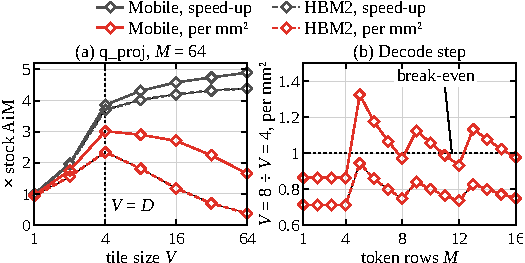
\includegraphics[width=\columnwidth]{figs/fig_vsweep.pdf}
  \caption{Tile size: (a)~q\_proj speed-up and throughput per logic mm$^2$ over stock AiM against $V$ at $M = 64$; (b)~$V = 8$ over
  $V = 4$, decode-step throughput per logic mm$^2$ against $M$.}
  \label{fig:vsweep}
\end{figure}

% sources-of-gain table (D-35; generated by scripts/make_tables.py, simulated rows, evaluation/dac_2x2 Sec. 2i):
% placement checked on the float map after each build
\begin{table}[t]
  \caption{Useful-MAC utilization from stock AiM to CoDe, one source at a time.}
  \label{tab:umac_src}
  \centering
  \footnotesize
  \setlength{\tabcolsep}{4pt}
  % generated by scripts/make_tables.py from evaluation/dac_2x2/figures/tab_umac_src_steps.csv (usrc_steps ids, simulated rows, layer, M = 8); do not edit
\begin{tabular}{@{}lccccc@{}}
\toprule
Design & \UMAC & \fMAC & $U$ & \multicolumn{2}{c@{}}{Speedup} \\
\cmidrule(l){5-6}
 & & & & step & cumul. \\
\midrule
\multicolumn{6}{@{}l}{\emph{Mobile:} Llama-2-7B, $V = 8$} \\
Stock AiM & 0.25 & 0.776 & 0.194 & -- & 1.00 \\
Row reuse only & 0.25 & 0.965 & 0.241 & 1.24 & 1.24 \\
\textbf{CoDe} & 1.00 & 0.843 & 0.843 & 3.49 & 4.35 \\
\midrule
\multicolumn{6}{@{}l}{\emph{Server:} Llama-3.1-8B, $V = 4$} \\
Stock AiM & 0.25 & 0.771 & 0.193 & -- & 1.00 \\
Row reuse only & 0.25 & 0.887 & 0.222 & 1.15 & 1.15 \\
\textbf{CoDe} & 1.00 & 0.739 & 0.739 & 3.33 & 3.83 \\
\bottomrule
\end{tabular}

\end{table}

% Conclusion: five moves (claim, key idea, what was done, one number, outlook); ~115 words; no cite, no ref.
\section{Conclusion}
\label{sec:conclusion}

% sources-of-gain table (D-35; generated by scripts/make_tables.py, simulated rows, evaluation/dac_2x2 Sec. 2i):
% defined here, after the Conclusion heading, so that it lands at the top of p. 11 R and not in Fig. 9's column
% (one float per column); placement checked on the float map after each build
\begin{table}[t]
  \caption{Useful-MAC utilization from stock AiM to CoDe, one source at a time.}
  \label{tab:umac_src}
  \centering
  \footnotesize
  \setlength{\tabcolsep}{4pt}
  % generated by scripts/make_tables.py from evaluation/dac_2x2/figures/tab_umac_src_steps.csv (usrc_steps ids, simulated rows, layer, M = 8); do not edit
\begin{tabular}{@{}lccccc@{}}
\toprule
Design & \UMAC & \fMAC & $U$ & \multicolumn{2}{c@{}}{Speedup} \\
\cmidrule(l){5-6}
 & & & & step & cumul. \\
\midrule
\multicolumn{6}{@{}l}{\emph{Mobile:} Llama-2-7B, $V = 8$} \\
Stock AiM & 0.25 & 0.776 & 0.194 & -- & 1.00 \\
Row reuse only & 0.25 & 0.965 & 0.241 & 1.24 & 1.24 \\
\textbf{CoDe} & 1.00 & 0.843 & 0.843 & 3.49 & 4.35 \\
\midrule
\multicolumn{6}{@{}l}{\emph{Server:} Llama-3.1-8B, $V = 4$} \\
Stock AiM & 0.25 & 0.771 & 0.193 & -- & 1.00 \\
Row reuse only & 0.25 & 0.887 & 0.222 & 1.15 & 1.15 \\
\textbf{CoDe} & 1.00 & 0.739 & 0.739 & 3.33 & 3.83 \\
\bottomrule
\end{tabular}

\end{table}

% P:conc-summary
Skinny GEMMs keep LLM decoding memory-bound on mobile platforms and edge servers, and prior DRAM PIM paces every
multiply--accumulate (MAC) by a DRAM command. This paper argues that DRAM timing bounds column accesses, not MACs on a
latched column. The key to CoDe is to decouple MAC timing from DRAM command timing: one column command feeds many processing-unit beats over a tile
of tokens. We build CoDe on each rival's own memory. On LPDDR5-6400, CoDe matches LP-Spec-style's decoding speed
with 1.87$\times$ its throughput per logic mm$^2$; on HBM2, CoDe decodes batches 1.68$\times$ faster than P3-LLM-style. Since a
column's beats follow from its period and the clock alone, the decoupling carries over to any DRAM whose column
outlasts one beat.


\bibliographystyle{IEEEtran}
\bibliography{refs}

\end{document}
